%%%% 2D Skewness Example %%%%%%
\subsection{Impact of Skewness on Accuracy}\label{ex:skewness}
In this example, we demonstrate the key point of this study: the magnitude of skewness between QoI maps impacts accuracy by orders of magnitude, and thus in optimizing the choice of a QoI map, it is in our interest to pursue the minimization of skewness.
This is especially true in problems where the number of random samples we are permitted to use is constrained by the computational cost of model evaluations.

%Thus, any map can be thought of as a piecewise-defined linear map, and the results we present in this example, while applying to all of $\pspace$ in these cases, can be applied solely to the support of each local linear approximation.
%Capturing the geometry of sets (improving accuracy) on each of these subdomains thus guarantees a desired result on the entirety of the domain.

To illustrate this point, we first define the linear maps
\begin{equation}\label{eq:qmap2}
\qspace_S := \left \lbrace Q^{(s)} =  \mat{cc}{1 & 0 \\ \sqrt{s^2 - 1}& 1 } \right \rbrace_{s\in S},
\end{equation}
for $S=\set{1,2,4}$ because they allow us to control the global skewness (since it is equal to local skewness in a linear map) while preserving the measures of sets between $\pspace$ and $\dspace$.
More specifically, the support of the solution to the SIP associated with each QoI map has equal $\mu_\pspace$-measure, which isolates the impact of accuracy solely to the skewness of the QoI map.
% We show what the component row vectors of these maps in Figure~\ref{fig: skewmapvecs} and note the skewness is determined by the ratio of the magnitude of the black line to its projection onto the vertical axis (and each of these projects directly on to the unit vector).
The skewness of these maps is given by the index $s$, so $Q^{(1)}$ is $1$, the skewness of $Q^{(2)}$ is $2$, and $S_{Q^{(4)}} = 4$.

% The maps chosen for this example are expository ones that provide valuable insight despite their simplicity.
% For example, when solving many physics-based problems, local linear approximations are often used to simplify model evaluation and guide optimization procedures.

%
% \begin{figure}[h]
% 	\begin{minipage}{.3\textwidth}
% 		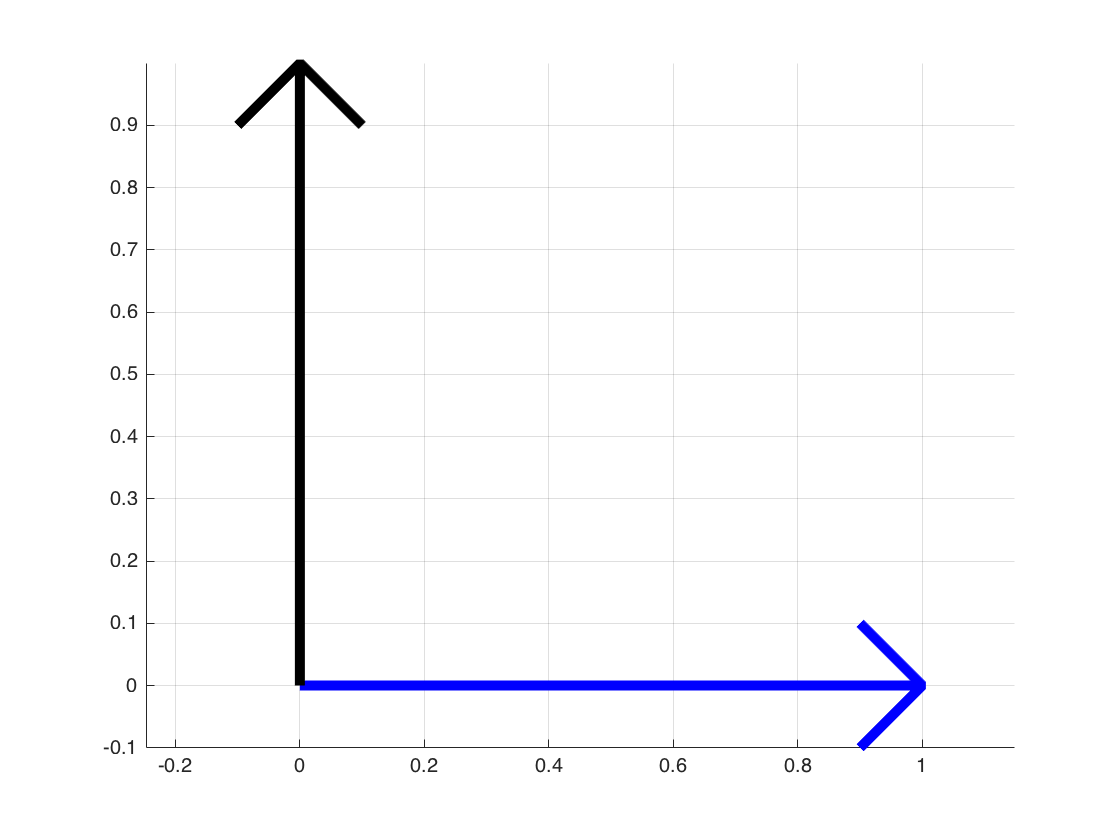
\includegraphics[width=\linewidth]{./images/vector_a.png}
% 	\end{minipage}
% 	\begin{minipage}{.3\textwidth}
% 		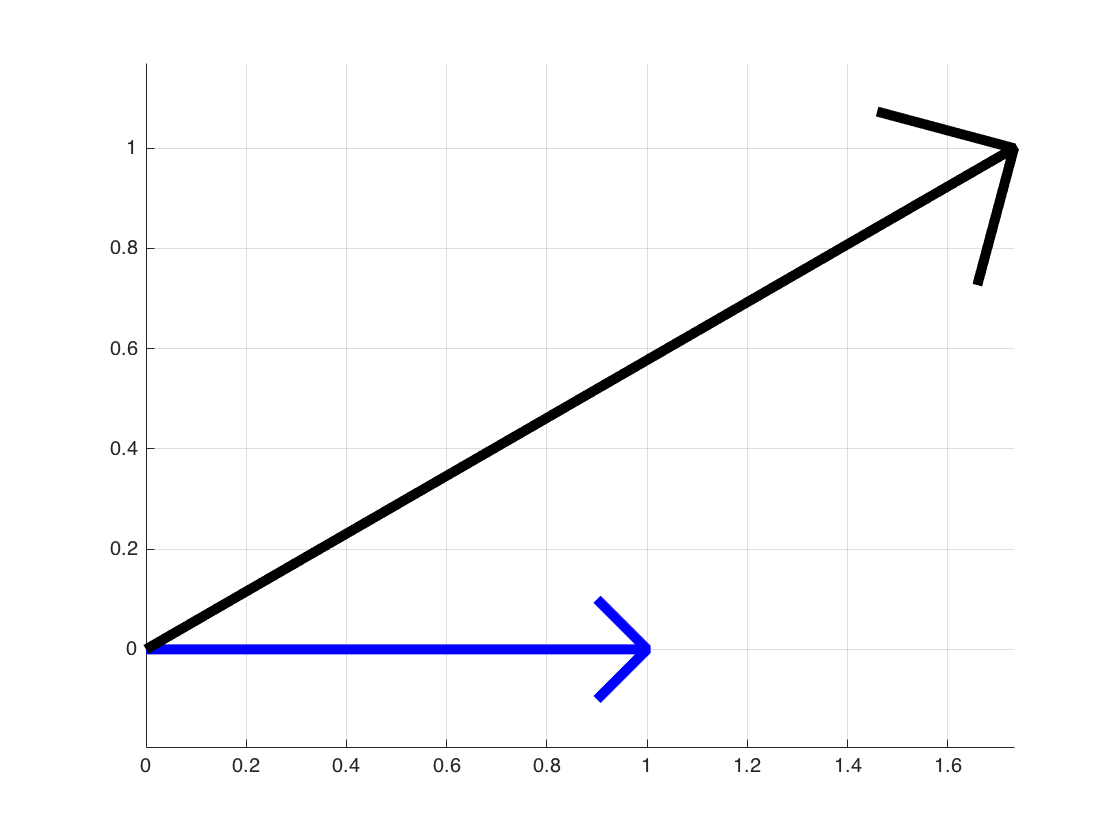
\includegraphics[width=\linewidth]{./images/vector_b.png}
% 	\end{minipage}
% 	\begin{minipage}{.3\textwidth}
% 		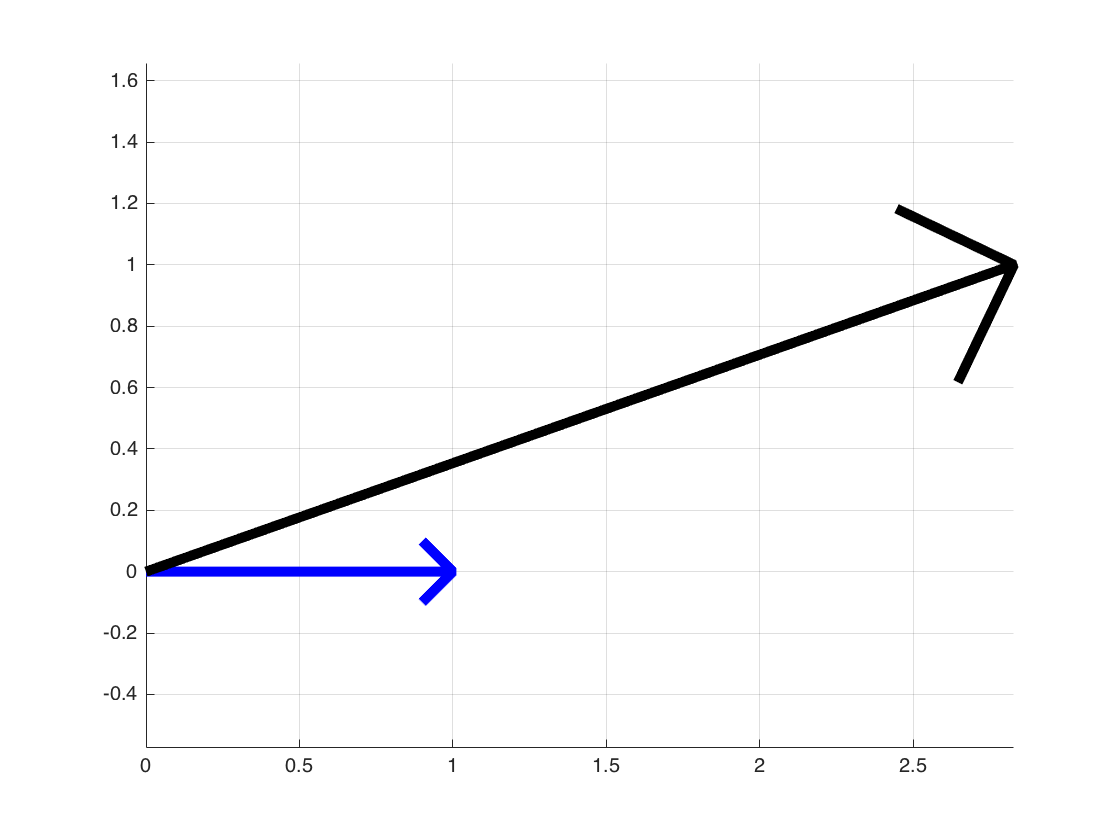
\includegraphics[width=\linewidth]{./images/vector_c.png}
% 	\end{minipage}
% \caption{(Left to right):  The component row-vectors of $Q^{(1)}$, $Q^{(2)}$, and $Q^{(4)}$. Our linear maps take $\RR^2$ to $\RR^2$ and can be visualized graphically as the component row-vectors of the matrices representing the transformation. The first row is highlighted in blue. The skewness is then simply equal to the reciprocal of the inverse sine of the angle between these vectors. }
% \label{fig: skewmapvecs}
% \end{figure}


\begin{figure}
\begin{minipage}{.5\textwidth}
\begin{table}[H]
\begin{tabular}{ c | c | c | c }
N & $Q^{(1)}$ & $Q^{(2)}$ & $Q^{(4)}$\\ \hline \hline
$200$ & $2.02E-01$ & $2.49E-01$ & $3.37E-01$\\ \hline

$400$ & $1.75E-01$ & $2.16E-01$ & $2.58E-01$\\ \hline

$800$ & $1.19E-01$ & $1.45E-01$ & $1.81E-01$\\ \hline

$1600$ & $8.23E-02$ & $9.67E-02$ & $1.29E-01$\\ \hline

$3200$ & $6.10E-02$ & $7.15E-02$ & $9.22E-02$\\ \hline

$6400$ & $3.96E-02$ & $5.47E-02$ & $6.39E-02$\\ \hline
\end{tabular}
\end{table}
\end{minipage}
\begin{minipage}{.45\textwidth}
		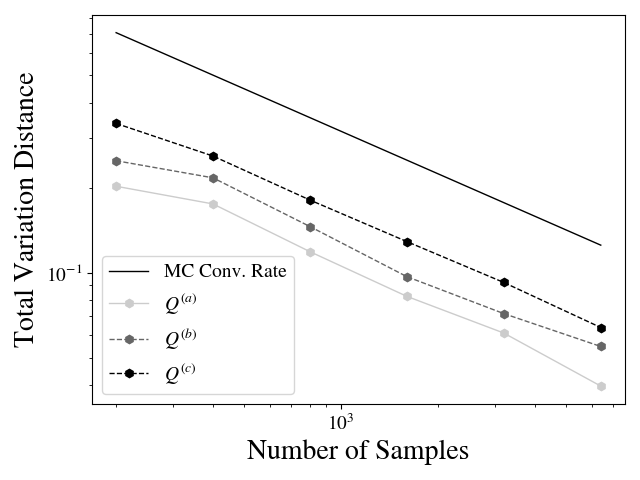
\includegraphics[width=\linewidth]{./images/Plot-reg_BigN_40000_reg_M_1_rand_I_100000}
\end{minipage}
\caption{The results of $d^2_\text{TV}(\PP_{\pspace, M, N}, \PP_{\pspace,\bar{N}})$.}
\label{fig:M1_2d}
\end{figure}

The displaced horizontal lines and accompanying table in Figure~\ref{fig:M1_2d} demonstrate that skewness has a direct impact on the number of samples required to achieve a particular value for the Total Variation distance.
By comparing adjacent columns in the table, it appears that if the ratio of skewness between two maps is 2, then the more-skewed map will require approximately twice as many random samples to approximate the set on a a well-resolved discretization with the same error tolerance.
We observe that the measure induced by $Q^{(1)}$ requires fewer than half the number of samples to be as accurately resolved as $Q^{(2)}$ does.
The effect is even more pronounced when compared against $Q^{(4)}$.

The fact we can achieve the same accuracy with fewer model evaluations provides a strong motivation for minimizing skewness and reinforces the results from \cite{BPW_2015}.
There, it was demonstrated that a similar relationship existed in the number of samples required to remove error in inverse set approximations quantified by the $\mu_\pspace$-measure of the {\em symmetric difference} of the inverse sets.
Rather than study the support of the distributions as was the focus in \cite{BPW_2015}, we turn our attention to a formal measure of accuracy for the densities or measures involved in the solution to the SIP.
We have shown that the skewness has an impact not only on the symmetric difference error, but also on the approximation error as measured by Total Variation.
